\section{Dielectric constant plot}
\noindent The relationship between $\epsilon_{r}$ and temperature $T$ was experimentally measured in Ref. [\citen{PhysRevB.19.3593}]. Below $\approx$ 4 K $\epsilon_{r}(T)$ remains constant at $\approx$ 23,000. The mean-field theorem derived in Ref. [\citen{PhysRev.86.118}] takes into account the quantum mechanical suppression of the low temperature ferroelectric phase transition in the crystal structure. Therefore the mean-field theory curve shown in Fig. (\ref{fig:epsilon_Tplot}) provides the closest approximation to the experimentally measured behaviour of $\epsilon_{r}(T)$.  

\begin{figure}[t]
\centering
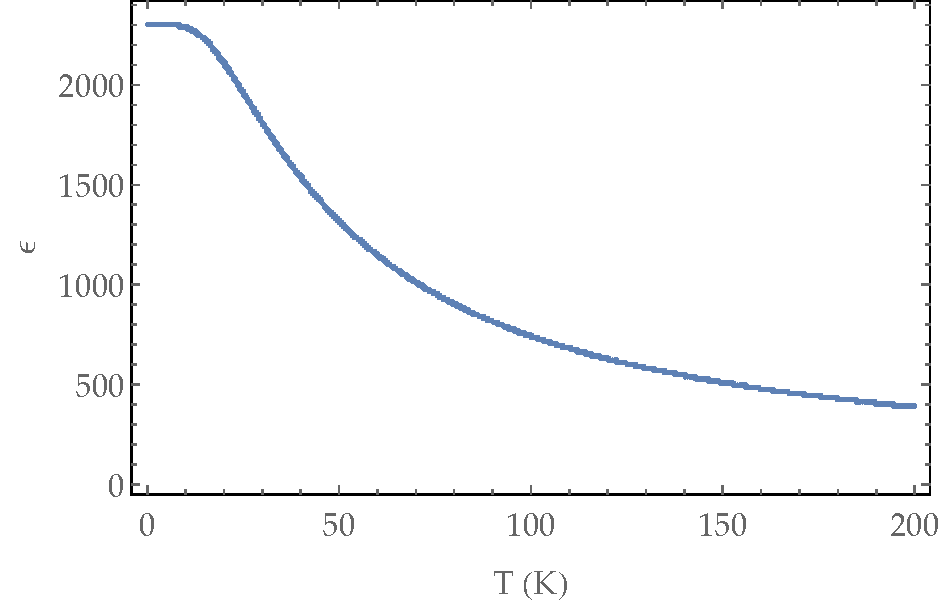
\includegraphics[height=0.32\textwidth,keepaspectratio]{epsilon_Tplot}
\caption{\label{fig:epsilon_Tplot}The quantum mean-field approximation of $\epsilon_{r}$ vs. $T$.}
\end{figure}

\section{\label{sec:Simulation}Simulation}
The numerical simulations completed to aid in the design of the varactors are discussed and presented in the following sections. 

\subsection{\label{varactorimpedancematching}Varactor impedance matching}
\noindent This section of the report outlines the numerical calculations completed to determine the values of the varactors required to enable impedance matching of the circuit. Firstly, to obtain an estimate of the magnitude of varactor values required, the $\textit{L-section  matching}$ derivation from Pozar [\citep{pozar2004microwave}] was employed. Following results obtaining those preliminary results a more detailed investigation of was conducted. The ranges of $C_{v1}$ and $C_{v2}$ investigated to determine the dynamic range. The results of these calculations are provided in Section \ref{subsubsec:L-sectionmatching} and \ref{subsubsec:Heuristicvaractoroptimisation}. The circuit components shown in Fig. (!PLEASE ENTER CIRCUIT DIAGRAM REFERENCE!!) are estimated as follows: $C_{p}=$, $R_{Loss}=15$ $\Omega$, $R_{Q}=1$ M$\Omega$, $C_{Q}=1$ fF. The inductor value of $L= 255$ nH was used through analytical calculations. However, the closest available inductor was $L =270$ nH.

\subsubsection{\label{subsubsec:L-sectionmatching}L-section matching}
\noindent Pozar [\citen{pozar2004microwave}] simplifies the device circuit as shown in Fig. (fig:L-sectionmatching) to three components written in terms of impedance. These three components include the two varactors and the load impedance $Z_{L}$. The complex impedance $Z_{L}$ is expressed as

\begin{equation}
\label{eq:compleximpedance}
Z_{L}=R_{L}+i X_{L},
\end{equation}


\noindent where the aim of impedance matching is to match $Z_{L}$ to a characteristic impedance $Z_{0}=$50 $\Omega$ whilst removing the imaginary component by setting $X_{L}=0$. Therefore to satisfy the impedance matching condition

\begin{equation}
\label{eq:compleximpedance}
\frac{1}{Z_{0}}=\frac{1}{iB}+\frac{1}{RL + i(X+X_{L})},
\end{equation}

\noindent then solving for $X$ and $B$ gives

\begin{equation}
\label{eq:Xsolved}
X=\pm \sqrt{R_{L}(Z_{0} − R_{L})}-X_{L},
\end{equation}
\begin{equation}
\label{eq:Bsolved}
B=\pm \frac{\sqrt{(Z_{0} − R_{L})/R_{L}}}{Z_{0}}.
\end{equation}

\noindent Plugging in the estimated component values for 600 MHz operation provides the results $C_{v1}=4.63 pF$ and $C_{v2}=8.19 pF$ which enable impedance matching for this circuit.  

\begin{figure}[t]
\centering
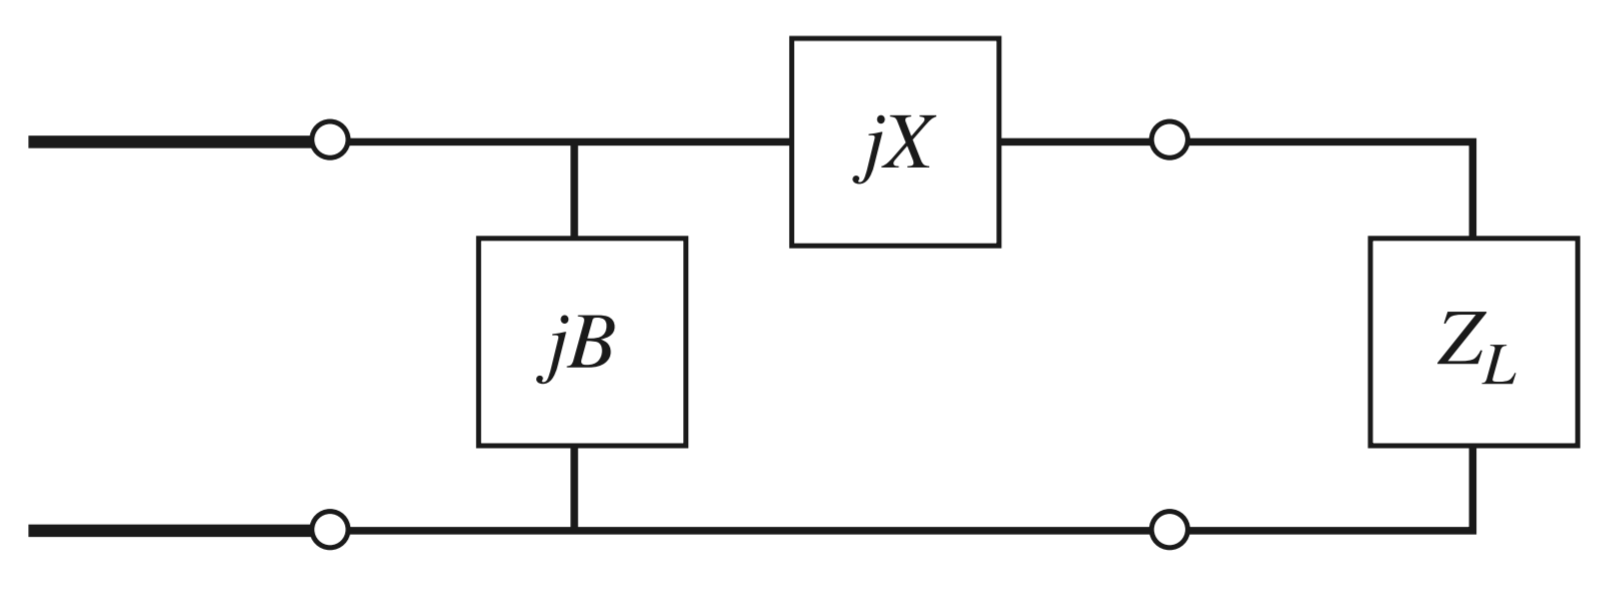
\includegraphics[height=0.2\textwidth,keepaspectratio]{L-sectionmatching}
\caption{\label{fig:L-sectionmatching} The simplified impedance matching and quantum dot device circuit\citep{pozar2004microwave}.}
\end{figure}

\subsubsection{\label{subsubsec:Heuristicvaractoroptimisation}Heuristic varactor optimisation}
\noindent The particle swarm optimisation [\citen{488968}] approach was taken to determine the circuit resonance tune-ability. Initially $C_{v2}$ was set to $8.19$ nF and sweeping $C_{v1}$ determined the dynamic range of 3-30 pF. The resonances range between 583-623 MHz providing a tune-ability around $f_{0}=600$ MHz of $\approx \pm 20$ MHz. Therafter, $C_{v2}$ is tuned to maximise impedance matching for $\left | R\right |$ < 0.02. For the dynamic range of $C_{v1}$ impedance matching is achieved where $C_{v2}$ ranges between 6.5-10.5 pF. For $C_{v1}=4.63$ pF, $f_{0}=600$ MHz and impedance matching is optimised for $C_{v2}=8.19$ nF. These values are in agreement with the results presented in Section \ref{subsubsec:L-sectionmatching}. 

Additionally, varying the resistive loss of the circuit between $R_{Loss}=10-20$ $\Omega$ has no significant effect of $f_{0}$ and the range of $C_{v2}$ enables impedance matching re-optimisation. However, the 15 nH difference between the simulated inductor value and the component available in the laboratory is significant. This is due to the nonlinear relationship between $C_{v1}$ and $f_{0}$ shown in Fig.(\ref{fig:f_0vsC_v1}). Consequently, $f_{0}$ is shift to 580 MHz which greatly limits the ability to tune $f_{0}$ using $C_{v1}$.  

    
\begin{figure}[t]
\centering
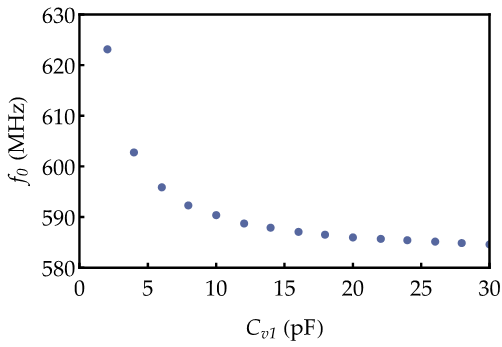
\includegraphics[height=0.3\textwidth,keepaspectratio]{f_0vsC_v1}
\caption{\label{fig:f_0vsC_v1} $f_{0}$ vs. $C_{v1}$.}
\end{figure}


\subsubsection{\label{subsec:Varactorgeometry}Varactor geometry}
The varactor geometry chosen to assist ease of fabricated was an interdigitated design \citep{PhysRevB.19.3593}. Analytical simulation of the interdigitated varactor was completed using the model provided by Igreja et at. [\citep{Igreja2004AnalyticalStructure}]. The capacitance values calculated from this model were used to inform the dimensions of the area etched by electron-beam lithography. Thereafter, the determined capacitance values were cross-checked using a finite element software package. 

The analytical results were found to significantly differ from the capacitance values derived through COMSOL simulation. Upon investigation of each method it was determined there was a mistake in the analytical model which resulted in an increase in the capacitance values by a factor of two. Unfortunately this error was not noted in time to update the etching dimensions so devices were fabricated with a larger capacitance than anticipated. The value of $\epsilon_{r}$ for the STO was assumed to be 23000.   

\subsubsection{\label{subsubsection:interdigitedelectrodemodel}Interdigited electrode model}
The model developed to compute the capacitance of an interdigitated varactor can be applied to structures when the number of electrode fingers $N$ are >3 such that 
\begin{equation}
\label{eq:capacitanceinterdigited}
C=(N-3) \frac{C_{I}}{2}+2\frac{C_{I}C_{E}}{C_{I}+C_{E}}.
\end{equation}

\noindent The capacitance of the an outer electrode relative to ground is given as $C_{E}$ while $C_{I}$ is half the capacitance of an inner electrode. This model makes the assumption of negligible electrode thickness compared to the electrode width $W$. This condition is satisfied for the fabricated varactors. Therefore, the capacitance greatly depends on the metalisation ratio
\begin{equation}
\label{eq:metalisationratio}
\eta =\frac{W}{W+G}
\end{equation}

where the width of the electrode gap is $G$. Combining the contribution of capacitance from the STO sample and air determines the contribution from air is negligible. 

For the varactor dimensions given in Table \ref{tab:varactordimensions} the values of $C_{v1}=30.3$ pF and $C_{v2}=14.8$ pF were initially outputted and used to fabricate the devices. However, following the correction to the analytical model the computed varactor capacitances are presented in Table. \ref{tab:varactordimensions}. In Ref. [\citep{Igreja2004AnalyticalStructure}] the model was verified by comparison using ANSYS software for computation of a $N=4$ interdigitated capacitor. The difference in results was 1.4 \% for a pF-scale capacitor.    

\begin{table}[h!]
  \begin{center}
    \caption{The varactor geometric dimensions and corrected capacitance values.}
    \label{tab:varactordimensions}
    \begin{tabular}{l|l|l|l|l|l|} % <-- Changed to S here.
      Varactor & N & $\mathcal{L}$ & W & G & Capacitance \\
       & & $\mu$m & $\mu$m & $\mu$m & pF \\
       \hline
       $C_{v1}$ & 8 & 50 & 25 & 5 & 68.3 \\
       $C_{v2}$ & 4 & 50 & 25 & 5 & 31.1\\
    \end{tabular}
  \end{center}
\end{table}


\begin{figure}[t]
\centering
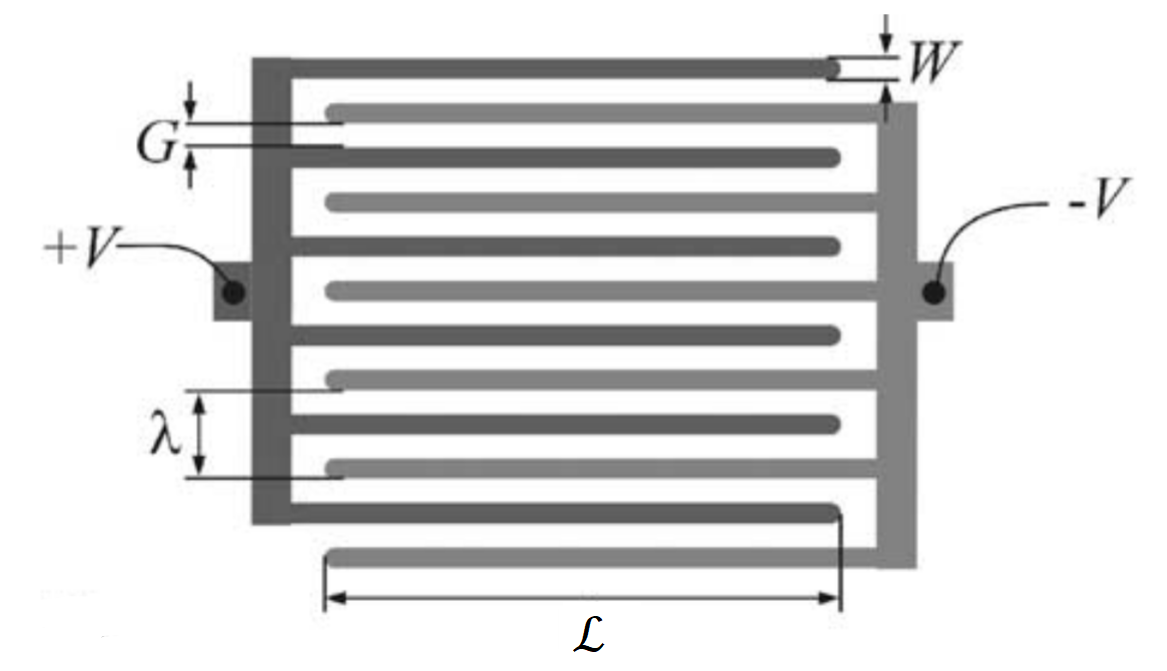
\includegraphics[height=0.3\textwidth,keepaspectratio]{interdigitalvaractor}
\caption{\label{fig:interdigitalvaractor} Varactor electrode geometry where $W$, $G$ and $\mathcal{L}$ provide the electrode width, gap size and length, respectively. \citep{Igreja2004AnalyticalStructure}.}
\end{figure}

\subsubsection{\label{subsubsec:COMSOLsimulation}COMSOL simulation}
The multi-physics software package COMSOL was utilised to provide an alternative means to calculate and verify the values of $C_{v1}$ and $C_{v2}$ for the interdigitated electrode geometry. The simple parallel plate capacitor tutorial [\citep{COMSOLtut}]] was adapter to allow the electrostatic properties of the interdigitated varactors to be investigated. The geometric electrode design generated in KLayout to aid etching the substrate was imported into COMSOL. The value of $\epsilon_{r}$ for the metal electrodes is approximated as 1 \citep{PhysRevB.6.4370}. 

User defined meshing was applied to the device as shown in Fig. (\ref{fig:varactormeshing}) where the meshing chosen determines the precision of the density of points in the simulation. The COMSOL derived values of $C_{v1}= 94$ pF and $C_{v2}= 44$ pF do not compare closely with the results shown in Table \ref{tab:varactordimensions}. However, the derived values of capacitance were observed to dependent strongly on the meshing applied resulting in a factor of two increase in capacitance for a coarse meshing applied between the electrodes. 

Additionally, for the example meshing shown in Fig. (\ref{fig:varactormeshing}) the simulated electric field is shown in Fig. (\ref{fig:electricfieldvectors}). This suggests the electric field is not modelled sufficiently with the current meshing. However, as the density of meshing increases the computational power required to complete the simulation increases. The time and memory required to run the COMSOL simulation are regarded as the limiting factors to improve the accuracy of the capacitance values outputted using this method. Measurement of the fabricated impedance matching circuit will allow properties of the varactors to be determined. This will further aid in gaining confidence in which model provides the most accurate results to advise future interdigitated capacitor fabrication.   




\begin{figure}[b]
\centering
\begin{subfigure}[b]{0.45\textwidth}
   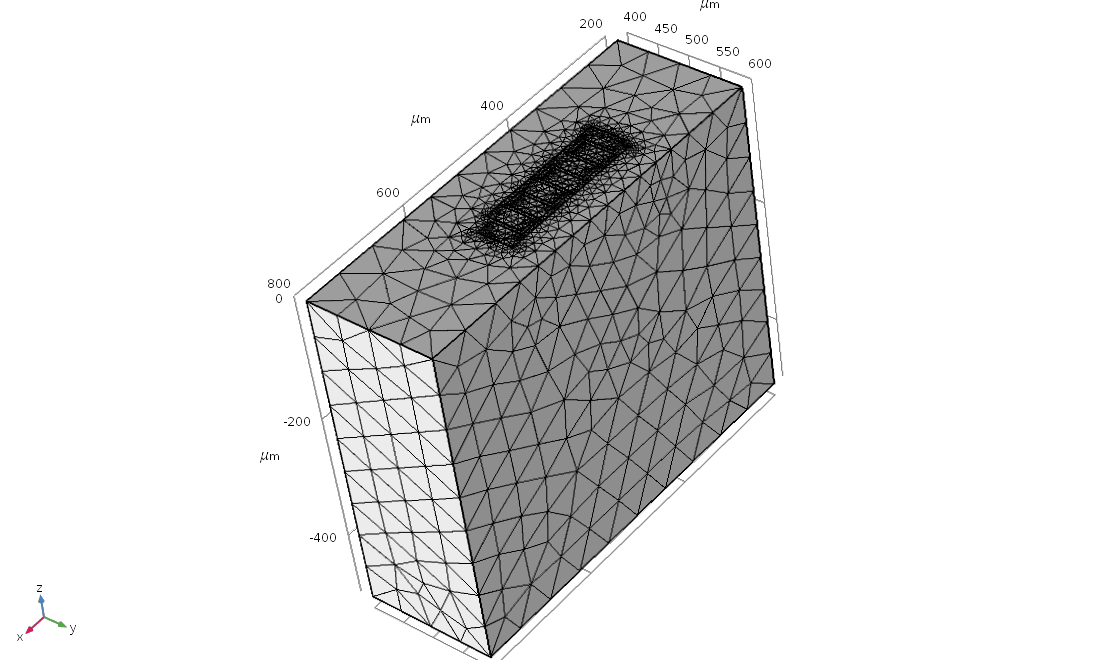
\includegraphics[width=1\linewidth]{varactormeshing}
	\caption{\label{fig:varactormeshing}}
\end{subfigure}
\begin{subfigure}[b]{0.45\textwidth}
   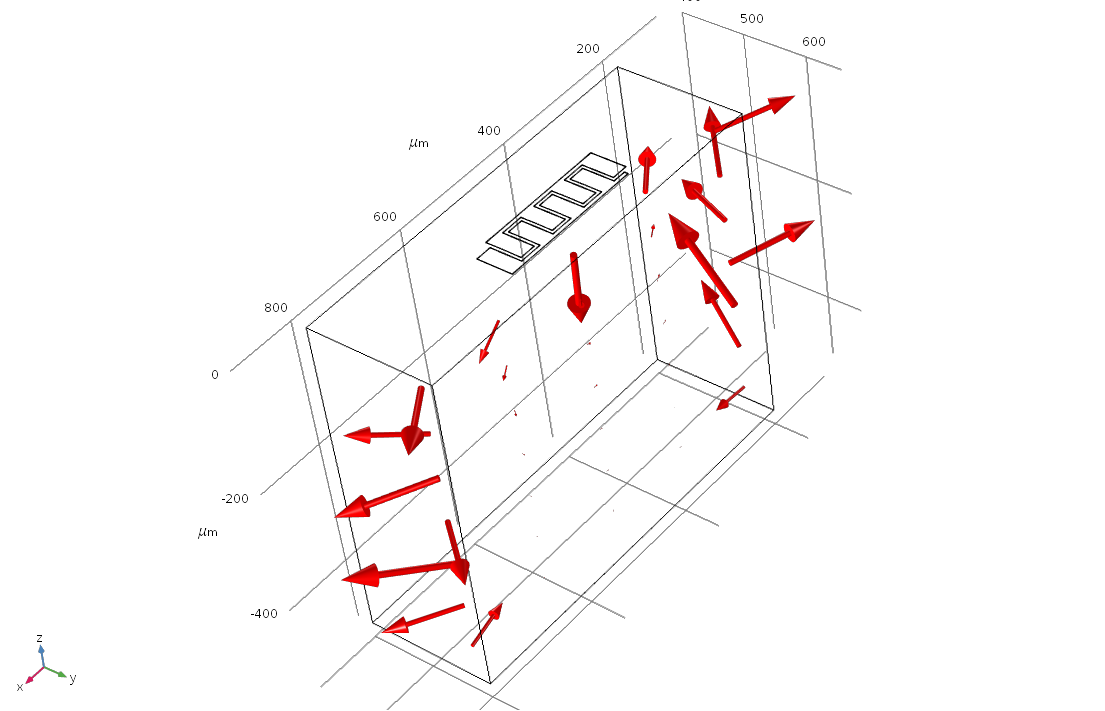
\includegraphics[width=1\linewidth]{electricfieldvectors}
	\caption{\label{fig:electricfieldvectors}}
\end{subfigure}
\caption[]{(a) COMSOL meshing applied to $C_{v1}$. (b) The simulated electric field for $C_{v1}$.}
\end{figure}









